%%%%%%%%%%%%%%%%%%%%%%%%%%%%%%%%%%%%%%%%%
% Beamer Presentation
% LaTeX Template
% Version 2.0 (March 8, 2022)
%
% This template originates from:
% https://www.LaTeXTemplates.com
%
% Author:
% Vel (vel@latextemplates.com)
%
% License:
% CC BY-NC-SA 4.0 (https://creativecommons.org/licenses/by-nc-sa/4.0/)
%
%%%%%%%%%%%%%%%%%%%%%%%%%%%%%%%%%%%%%%%%%

%----------------------------------------------------------------------------------------
%	PACKAGES AND OTHER DOCUMENT CONFIGURATIONS
%----------------------------------------------------------------------------------------

\documentclass[
	11pt, % Set the default font size, options include: 8pt, 9pt, 10pt, 11pt, 12pt, 14pt, 17pt, 20pt
	%t, % Uncomment to vertically align all slide content to the top of the slide, rather than the default centered
	%aspectratio=169, % Uncomment to set the aspect ratio to a 16:9 ratio which matches the aspect ratio of 1080p and 4K screens and projectors
]{beamer}

\graphicspath{{Images/}{./}} % Specifies where to look for included images (trailing slash required)

\usepackage{booktabs} % Allows the use of \toprule, \midrule and \bottomrule for better rules in tables

\usepackage{listings}
\usepackage{siunitx}
\usepackage{tikz}
\usetikzlibrary{arrows.meta}
\usetikzlibrary{patterns}
%----------------------------------------------------------------------------------------
%	SELECT LAYOUT THEME
%----------------------------------------------------------------------------------------

% Beamer comes with a number of default layout themes which change the colors and layouts of slides. Below is a list of all themes available, uncomment each in turn to see what they look like.

\usetheme{Madrid}

%----------------------------------------------------------------------------------------
%	SELECT COLOR THEME
%----------------------------------------------------------------------------------------

% Beamer comes with a number of color themes that can be applied to any layout theme to change its colors. Uncomment each of these in turn to see how they change the colors of your selected layout theme.

%\usecolortheme{albatross}
%\usecolortheme{beaver}
%\usecolortheme{beetle}
%\usecolortheme{crane}
%\usecolortheme{dolphin}
%\usecolortheme{dove}
%\usecolortheme{fly}
%\usecolortheme{lily}
%\usecolortheme{monarca}
%\usecolortheme{seagull}
%\usecolortheme{seahorse}
%\usecolortheme{spruce}
%\usecolortheme{whale}
%\usecolortheme{wolverine}

%----------------------------------------------------------------------------------------
%	SELECT FONT THEME & FONTS
%----------------------------------------------------------------------------------------

% Beamer comes with several font themes to easily change the fonts used in various parts of the presentation. Review the comments beside each one to decide if you would like to use it. Note that additional options can be specified for several of these font themes, consult the beamer documentation for more information.

\usefonttheme{default} % Typeset using the default sans serif font
%\usefonttheme{serif} % Typeset using the default serif font (make sure a sans font isn't being set as the default font if you use this option!)
%\usefonttheme{structurebold} % Typeset important structure text (titles, headlines, footlines, sidebar, etc) in bold
%\usefonttheme{structureitalicserif} % Typeset important structure text (titles, headlines, footlines, sidebar, etc) in italic serif
%\usefonttheme{structuresmallcapsserif} % Typeset important structure text (titles, headlines, footlines, sidebar, etc) in small caps serif

%------------------------------------------------

%\usepackage{mathptmx} % Use the Times font for serif text
\usepackage{palatino} % Use the Palatino font for serif text

%\usepackage{helvet} % Use the Helvetica font for sans serif text
\usepackage[default]{opensans} % Use the Open Sans font for sans serif text
%\usepackage[default]{FiraSans} % Use the Fira Sans font for sans serif text
%\usepackage[default]{lato} % Use the Lato font for sans serif text

%----------------------------------------------------------------------------------------
%	SELECT INNER THEME
%----------------------------------------------------------------------------------------

% Inner themes change the styling of internal slide elements, for example: bullet points, blocks, bibliography entries, title pages, theorems, etc. Uncomment each theme in turn to see what changes it makes to your presentation.

%\useinnertheme{default}
\useinnertheme{circles}
%\useinnertheme{rectangles}
%\useinnertheme{rounded}
%\useinnertheme{inmargin}

%----------------------------------------------------------------------------------------
%	SELECT OUTER THEME
%----------------------------------------------------------------------------------------

% Outer themes change the overall layout of slides, such as: header and footer lines, sidebars and slide titles. Uncomment each theme in turn to see what changes it makes to your presentation.

%\useoutertheme{default}
%\useoutertheme{infolines}
%\useoutertheme{miniframes}
%\useoutertheme{smoothbars}
%\useoutertheme{sidebar}
%\useoutertheme{split}
%\useoutertheme{shadow}
%\useoutertheme{tree}
%\useoutertheme{smoothtree}

%\setbeamertemplate{footline} % Uncomment this line to remove the footer line in all slides
%\setbeamertemplate{footline}[page number] % Uncomment this line to replace the footer line in all slides with a simple slide count

%\setbeamertemplate{navigation symbols}{} % Uncomment this line to remove the navigation symbols from the bottom of all slides

\lstset{
	language=R,
literate={\$}{{\textcolor{blue}{\$}}}1
}

%----------------------------------------------------------------------------------------
%	PRESENTATION INFORMATION
%----------------------------------------------------------------------------------------

\title[]{Analýza vazby mezi teplotou vzduchu ve standardní výšce a v hladině bylinného patra v závislosti na meteorologických podmínkách} % The short title in the optional parameter appears at the bottom of every slide, the full title in the main parameter is only on the title page

\author[]{Vojtěch Klimeš} % Presenter name(s), the optional parameter can contain a shortened version to appear on the bottom of every slide, while the main parameter will appear on the title slide

\institute[MFF UK]{Univerzita Karlova} % Your institution, the optional parameter can be used for the institution shorthand and will appear on the bottom of every slide after author names, while the required parameter is used on the title slide and can include your email address or additional information on separate lines

\date[5.9.2023]{Obhajoba bakalářské práce} % Presentation date or conference/meeting name, the optional parameter can contain a shortened version to appear on the bottom of every slide, while the required parameter value is output to the title slide

%----------------------------------------------------------------------------------------

\begin{document}

%----------------------------------------------------------------------------------------
%	TITLE SLIDE
%----------------------------------------------------------------------------------------

\begin{frame}
	\titlepage % Output the title slide, automatically created using the text entered in the PRESENTATION INFORMATION block above
\end{frame}

%----------------------------------------------------------------------------------------
%	TABLE OF CONTENTS SLIDE
%----------------------------------------------------------------------------------------

% The table of contents outputs the sections and subsections that appear in your presentation, specified with the standard \section and \subsection commands. You may either display all sections and subsections on one slide with \tableofcontents, or display each section at a time on subsequent slides with \tableofcontents[pausesections]. The latter is useful if you want to step through each section and mention what you will discuss.

\begin{frame}
	\frametitle{Obsah} % Slide title, remove this command for no title
	
	\tableofcontents % Output the table of contents (all sections on one slide)
	%\tableofcontents[pausesections] % Output the table of contents (break sections up across separate slides)
\end{frame}

%----------------------------------------------------------------------------------------
%	PRESENTATION BODY SLIDES
%----------------------------------------------------------------------------------------

\section{Úvod} % Sections are added in order to organize your presentation into discrete blocks, all sections and subsections are automatically output to the table of contents as an overview of the talk but NOT output in the presentation as separate slides

%------------------------------------------------

\subsection{Problematika}

\begin{frame}
	\frametitle{Problematika}
	\begin{itemize}
		\item Teplota a jiné meteorologické podmínky jsou typicky měřeny standardizovanými meteorologickými stanicemi.
		\item Teploty ve $\SI{2}{m}$ nereflektují podmínky, v kterých žije většina organismů
		\item Lesní mikroklima je velmi odlišné od klimatu v okolí meteorologické stanice.
	\end{itemize}
\end{frame}

\begin{frame}
	\frametitle{Problematika}
Cílem této práce je analyzovat rozdíl mezi teplotami naměřenými v lesním porostu ve výšce $\SI{2}{m}$ nad zemí a v $\SI{15}{cm}$, resp. $\SI{0}{cm}$ nad zemí.
\end{frame}

\subsection{Klima nízko nad zemí}
\begin{frame}
	\frametitle{Klima nízko nad zemí}
\begin{figure}
\centering
	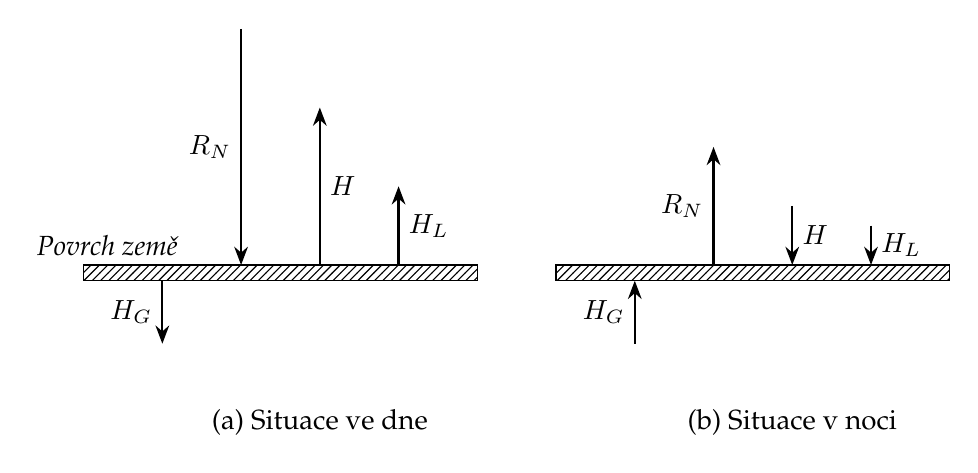
\begin{tikzpicture}
  % Part a: Day
  \draw (-1,0) -- (4,0);
  \draw[pattern=north east lines] (-1,0) rectangle (4,-0.2);
	\draw[-{Stealth},thick] (1,3) -- (1,0) node[midway,left] {$R_N$};
  \draw[-{Stealth},thick] (2,0) -- (2,2) node[midway,right] {$H$};
  \draw[-{Stealth},thick] (3,0) -- (3,1) node[midway,right] {$H_L$};
  \draw[-{Stealth},thick] (0,-0.2) -- (0,-1) node[midway,left] {$H_G$};
  \node at (2,-2) {(a) Situace ve dne};
	\node at (-0.7,0.25) {\textit{Povrch země}};

  % Part b: Night
  \begin{scope}[xshift=6cm]
    \draw (-1,0) -- (4,0);
    \draw[pattern=north east lines] (-1,0) rectangle (4,-0.2);
    \draw[-{Stealth},thick] (1,0) -- (1,1.5) node[midway,left] {$R_N$};
    \draw[-{Stealth},thick] (2,0.75) -- (2,0) node[midway,right] {$H$};
    \draw[-{Stealth},thick] (3,0.5) -- (3,0) node[midway,right] {$H_L$};
    \draw[-{Stealth},thick] (0,-1) -- (0,-0.2) node[midway,left] {$H_G$};
    \node at (2,-2) {(b) Situace v noci};
  \end{scope}
	\end{tikzpicture}
	\caption{Schéma ukazující rozdíl mezi tokem tepla v noci a přes den}
\label{fig:schema}
\end{figure}
\end{frame}

\begin{frame}
	\frametitle{Klima nízko nad zemí}
	\begin{itemize}
		\item Teplota dosahuje maxima 1 až 2 hodiny po maximální insolaci, minima v brzkých ranních hodinách.
		\item Teplotní gradienty v blízkosti vyhřátého povrchu můžou dosahovat vysokých hodnot ($\si{}{K/mm}$).
	\end{itemize}
\end{frame}

\subsection{Analýza faktorů ovlivňující teplotu vzduchu v lesním porostu}
%------------------------------------------------

\begin{frame}
	\frametitle{Topografie a struktura krajiny}
	Topografie ovlivňuje teploty v lesním porostu
	\begin{itemize}
		\item Okraj lesa
		\item Sklon svahu
		\item Nadmořská výška
		\item Údolí/hřeben
	\end{itemize}
\end{frame}

\begin{frame}
	\frametitle{Vegetace}
	Vegetační faktory ovlivňující teploty v lesním porostu
	\begin{itemize}
		\item Zápoj (otevřenost porostu)
		\item Plocha koruny stromů
		\item Procento plochy pokryté dřevinami
		\item Typ dřeviny
	\end{itemize}
\end{frame}

\begin{frame}
	\frametitle{Meteorologické podmínky}
	Vybrané sledované meteorologické podmínky
	\begin{itemize}
		\item Výška sněhu
		\item Oblačnost
		\item Půdní vlhkost
		\item Srážky
		\item Rychlost větru
		\item Insolace
	\end{itemize}
\end{frame}

%------------------------------------------------

\subsection{Použitá data}

\begin{frame}
	\frametitle{Použitá data}
	Stanice: Kvilda, Horská Kvilda, Churáňov, Borová Lada, Javoří Pila\\
	Celkově 157 čidel

	Maximální časový interval: 12.10.2019 - 19.5.2021
	\begin{figure}
		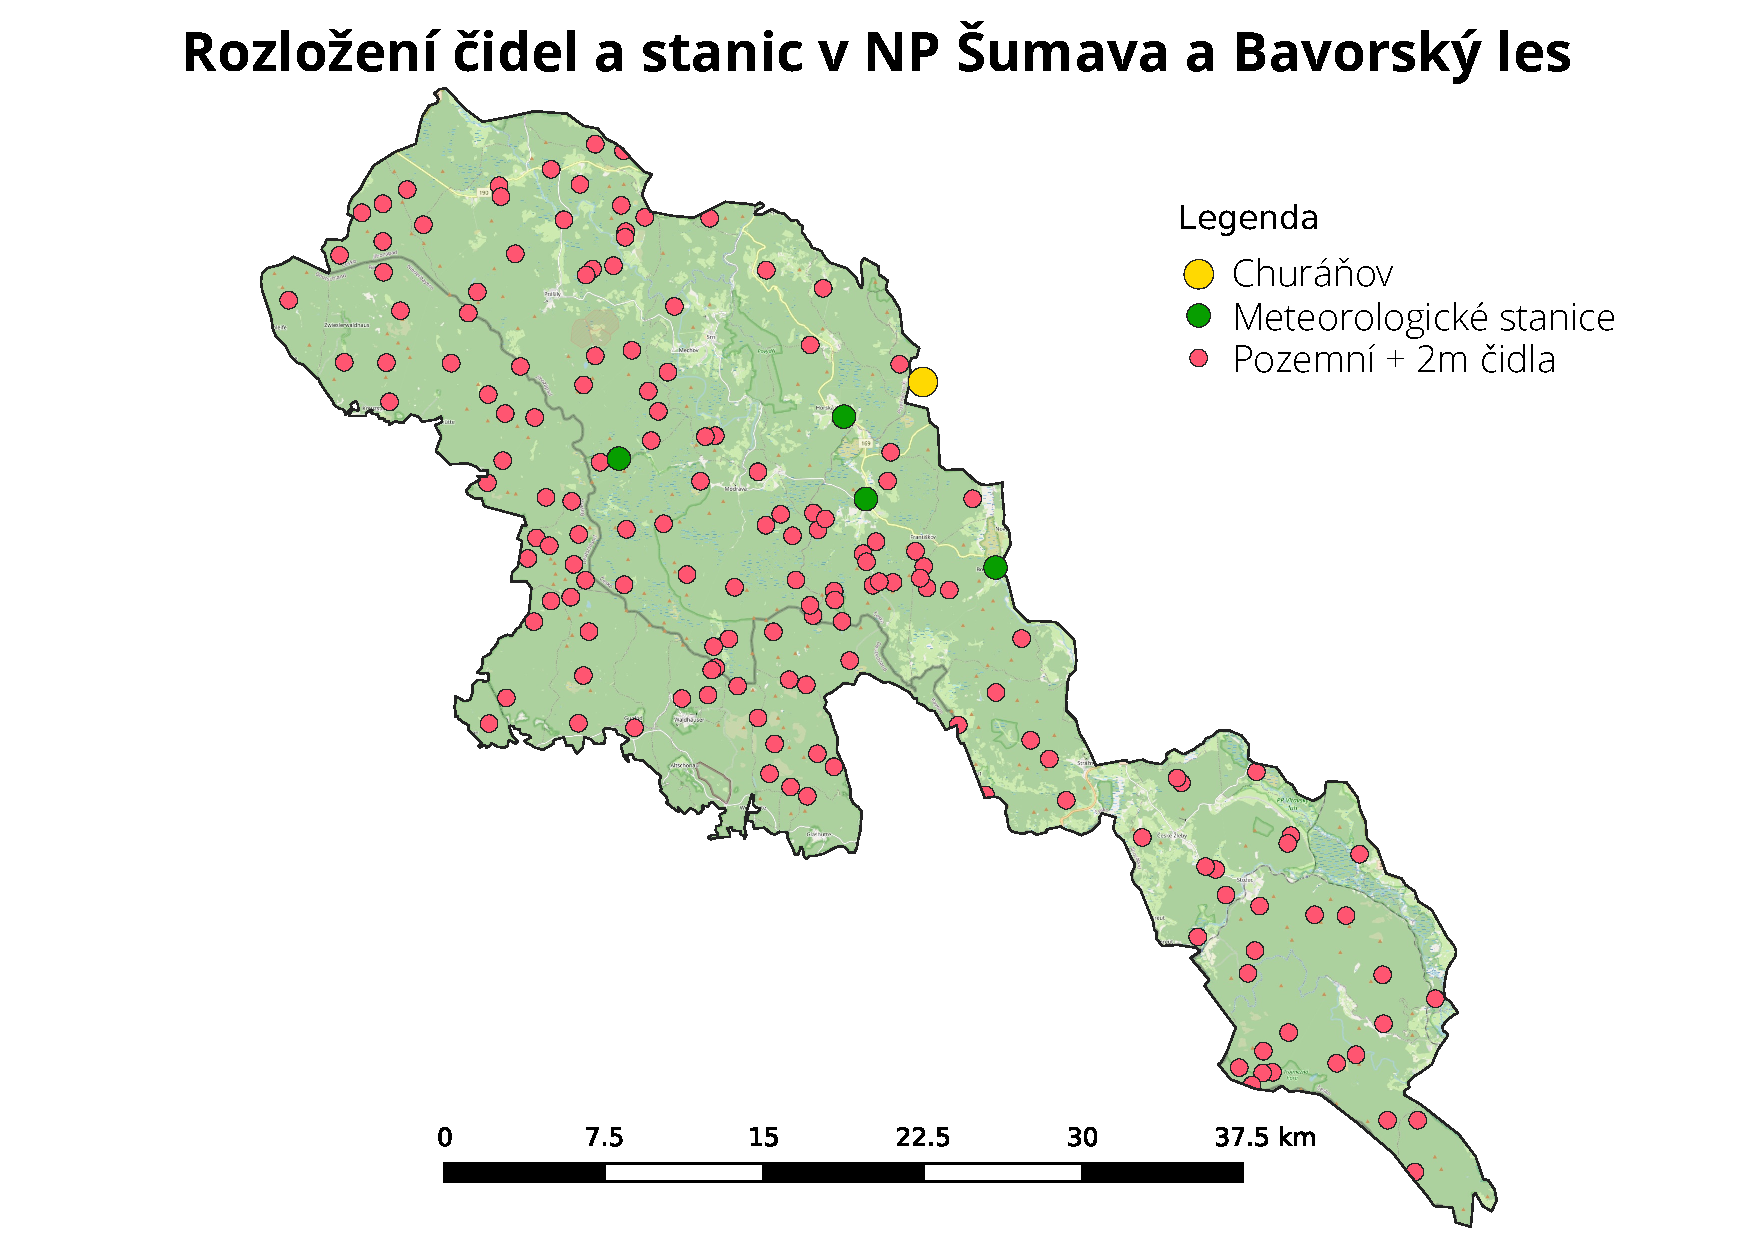
\includegraphics[width=0.7\linewidth]{rozlozenicidel.pdf}
	\end{figure}
\end{frame}

\begin{frame}
	\frametitle{Rozložení čidel v lesním porostu}
	\begin{figure}
		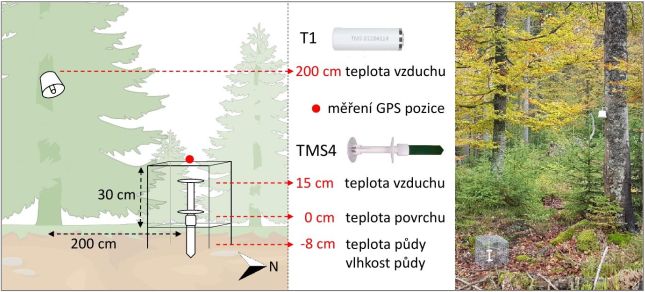
\includegraphics[width=0.9\linewidth]{sensor_closeup.png}
	\end{figure}
\end{frame}

%------------------------------------------------

\section{Metody a výsledky}

\subsection{Metody}
\frametitle{Statistické zpracování}
\begin{frame}
	\begin{itemize}
		\item Použijeme lineární modely se smíšenými efekty
		\begin{itemize}
			\item Náhodný efekt: identita čidla
			\item Fixní efekt: výška sněhu, oblačnost, vlhkost, srážky, rychlost větru, insolace
			\item Autokorelace se zbavýme pomocí ARMA modelu
		\end{itemize}
	\item Celkově spočteme 32 modelů 
		\begin{itemize}
				\item Maximální/minimální teploty
				\item $\SI{0}{cm}$/$\SI{15}{cm}$
				\item Celé období/teplé období/studené období
				\item Sníh jako kategorická proměnná
				\item $\Delta T_1 = T_{\text{zem}}-T_{2m}$ nebo $\Delta T_2 = \left|T_{\text{zem}}-T_{2m}\right|$
		\end{itemize}
	\end{itemize}
\end{frame}

%------------------------------------------------

\subsection{Výsledky a diskuze}

\begin{frame}
\frametitle{Ukázka výsledných modelů}
\begin{table}
\centering\footnotesize\sf
\begin{tabular}{lrrrrr}
\toprule
	Model & Max15all & Max15warm & Max15cold & Max15allc & Max15coldc \\
\midrule
	$R_m^2$ & $0.031$ & $0.098$ & $0.066$ & $0.032$ & $0.067$\\
	$R_c^2$ & $0.20$ & $0.51$ & $0.19$ & $0.20$ & $0.19$\\
\midrule
	Konstanta & $\SI{0.42(6)}{}$ & $\SI{-0.55(7)}{}$ & $\SI{0.96(7)}{}$ & $\SI{0.43(6)}{}$ & $\SI{0.99(7)}{}$\\
	Výška sněhu & $\SI{0.0045(7)}{}$ & - & $\SI{0.0031(7)}{}$ & $\SI{0.040(9)}{}$ & \textcolor{gray}{$\SI{0.005(9)}{}$}\\
	Oblačnost & $\SI{-0.041(8)}{}$ & $\SI{-0.16(1)}{}$ & $\SI{0.03(1)}{}$ & $\SI{-0.040(8)}{}$ & $\SI{0.03(1)}{}$\\
	Vlhkost & $\SI{-0.6(1)}{}$ & $\SI{2.2(1)}{}$ & $\SI{-2.4(2)}{}$ & $\SI{-0.6(1)}{}$ & $\SI{-2.4(2)}{}$\\
	Srážky & \textcolor{gray}{$\SI{0.002(2)}{}$} & $\SI{-0.04(1)}{}$ & \textcolor{gray}{$\SI{0.003(2)}{}$} & \textcolor{gray}{$\SI{0.002(2)}{}$} & \textcolor{gray}{$\SI{0.003(2)}{}$}\\
	Rychlost větru & $\SI{-0.0072(4)}{}$ & $\SI{-0.0034(7)}{}$ & $\SI{-0.0098(6)}{}$ & $\SI{-0.0072(4)}{}$ &$\SI{-0.0098(6)}{}$\\
	Insolace & $\SI{0.00042(1)}{}$ & $\SI{0.00065(1)}{}$ & $\SI{0.00029(2)}{}$ & $\SI{0.00042(1)}{}$ & $\SI{0.00028(2)}{}$\\
\bottomrule
\end{tabular}
\end{table}
\end{frame}

\begin{frame}
Hlavní závěry
	\begin{itemize}
		\item Výška sněhu má kladný vliv na rozdíl teplot
		\item Oblačnost a rychlost větru má záporný vliv
		\item Insolace má slabý kladný vliv, množství srážek je nejméně průkazný prediktor
		\item Půdní vlhkost má složitější vztah s rozdílem teplot
	\end{itemize}
Hlavní body diskuze
	\begin{itemize}
		\item Velká nevysvětlená variabilita
		\item Vzdálenost mezi čidly a stanicemi
		\item Zanedbání různé topografie a vegetace
		\item Krátké zpracovávané období
	\end{itemize}
\end{frame}


%----------------------------------------------------------------------------------------
%	CLOSING SLIDE
%----------------------------------------------------------------------------------------

\begin{frame}[plain] % The optional argument 'plain' hides the headline and footline
	\begin{center}
		{\Huge Konec prezentace}
	\end{center}
\end{frame}

%----------------------------------------------------------------------------------------

\begin{frame}[plain] % The optional argument 'plain' hides the headline and footline
	\frametitle{1. otázka oponenta}

Statistická významnost regresních koeficientů (tabulky 3.1 až 3.8) je podle textu odhadována na základě F-testu; F-test zavedený v kapitole 1.5.3 je nicméně určen pro test nulové hypotézy předpokládající nulovost všech koeficientů. Jak byla stanovena významnost pro individuální prediktory?

%Postupně byly testovaný prediktory ve stejném pořadí, což dělá funkce anova(). Byla použita ANOVA typu I, kde první prediktor bere všechnu variabilitu kterou mu může náležet. Píšeme to jako SS - sum of squares SS(A) pro prediktor A, SS(B|A) pro prediktor B. SS je jinak s^2 = 1/(n-1) \sum (y_i-\bar{y})^2. Snažíme se minimalizovat SSE - sum of squared estimate of errors, což je kvadrát residuálů modelu neboli nevysvětlených hodnot. 

%F statistika je podíl vysvětlené a nevysvětlené variance. Vysvětlená se vypočítá jako sum of squares of model (ještě něco se stupněma volnosti). Nevysvětlená variance je pak daná sum of squares of error tj to s těmi residuály a opět něco se stupněma volnosti. Takto otestuji první prediktor a pokračuju na další přičemž množství nevysvětlené variability mi postupně klesá. Nejlépe je to vysvětlené tady: http://facweb.cs.depaul.edu/sjost/csc423/documents/f-test-reg.htm (to je to původní vysvětlení ale snadno se to dá převést na to sequential sum of squares).
\end{frame}

\begin{frame}
F-test může sloužit k testování statistické významnosti koeficientů lineárního (smíšeného) modelu. Máme-li nulovou hypotézu, že všechny koeficienty modelu $\beta_i = 0\, \forall\ i$. Dále máme-li alternativní hypotézu $\exists\ j, \beta_j\neq 0$. Spočteme $F$ statistiku jako podíl vysvětlené a nevysvětlené variance. Následně spočteme pomocí statistického softwaru konfidenční interval $I$, jako $(1-\alpha)\cdot\SI{100}{\%}$, kde $\alpha = 0.05$. Zavrhneme nulovou hypotézu, pokud $F\notin I$ a určíme p-hodnotu. V programovacím jazyce \texttt{R} můžeme použít například funkci \texttt{anova}.
\end{frame}

\begin{frame}
	Použili jsme ANOVU typu I. \\
	$SSE = \sum_{i=1}^n(y_i-\hat{y}_i)^2$, $SSR = \sum_{i=1}^n(\hat{y}_i-\bar{y})^2$, $y_i$ je pozorovaná hodnota, $\hat{y}_i$ je predikovaná hodnota, $\bar{y}$ je průměr pozorovaných hodnot.\\

	%$SSR(\text{sníh})$, $SSR(\text{oblačnost}|\text{sníh}$), $SSR(\text{vlhkost}|\text{sníh},\text{oblačnost})$, ...

	$F_{\text{sníh}} = SSR(\text{sníh})/(SSE/(n-p))$, \\
	$F_{\text{oblačnost,sníh}} = (SSR(\text{oblačnost}|\text{sníh})-SSR(\text{sníh}))/(SSE/(n-p))$ ...\\
	V tabulce F hodnot najdeme pro stupně volnosti odpovídající hodnotu. Stanovíme $\alpha = 0.05$. \texttt{qf()}\\
	Určíme p-hodnotu pomocí statistického softwaru \texttt{pf()}.
\end{frame}

\begin{frame}[fragile]
\begin{lstlisting}[basicstyle=\tiny]
data(iris)

model1 <- lm(Sepal.Length ~ Sepal.Width, data = iris)
model2 <- lm(Sepal.Length ~ Sepal.Width + Petal.Length, data = iris)
model3 <- lm(Sepal.Length ~ Sepal.Width + Petal.Length + Petal.Width, data = iris)

SSE <- sum(model3$residuals^2)
SSR1 <- sum((predict(model1) - mean(iris$Sepal.Length))^2)
SSR2 <- sum((predict(model2) - mean(iris$Sepal.Length))^2)
SSR3 <- sum((predict(model3) - mean(iris$Sepal.Length))^2)
F1 <- (SSR1 / 1) / (SSE / (nrow(iris) - 4))
F2 <- ((SSR2 - SSR1) / 1) / (SSE / (nrow(iris) - 4))
F3 <- ((SSR3 - SSR2) / 1) / (SSE / (nrow(iris) - 4))
print(c(F1,F2,F3))
anova(model3)
\end{lstlisting}
\end{frame}

\begin{frame}[plain] % The optional argument 'plain' hides the headline and footline
	\frametitle{2. otázka oponenta}

Jaká metoda byla použita pro kalibraci modelů? (a konkrétně, bylo by možné volbou odlišné techniky neúspěšnou kalibraci jedné z modelových konfigurací, zmiňovanou na straně 42?)

%Jde o otázku na nastavení modelu při jeho výpočtu. Optimalizační funkce (optim v Rku?) methods() getAnywhere(), BFGS, quasi Newton method, zkusit změnit optimatlizační funkci a fungovalo/nefungovalo to

%Používám funkce lme balíčku nlme. Následně používám defaultní nastavení. Hodnoty jsou nalezené aby splňovaly maximalizaci "restricted log likelihood" tj REML. Hodnoty jsou hledány pomocí základní funkce optim() a defaultním parametrem neboli metodou BFGS což je kvazi-Newtonovská metoda k hledání vhodných hodnot.

%REML -> MLE neboli maximum likelihood estimation je hledání parametrů tak aby byla maximalizovaná likelihood function což je funkce parametru který se snažíme zjistit v závislosti na pozorování, která nám dává pravděpodobnost naměření našich dat při daném parametru. REML je modifikace která bere v potaz množství fixních efekt lme a ztrácí jeden stupeň volnosti za každý fixní efekt.

%BFGS je O(n^2) metoda. Obyčejná Newtonova metoda hledá minimum diferencovatelné funkce pomocí Taylorova rozvoje do druhého řádu v nějakém bodě a pak posouváním se do minima toho Taylorova rozvoje a tak dále pokračováním. BFGS je vylepšení kde hledáme řešení rovnice $B_k\vec{p}_k=-\nabla f(\vec{x}_k)$, kde $B_k$ je Hessián v bodě $\vec{x}_k$, napravo je gradient funkce a $\vec{p}_k$ je 
\end{frame}

\begin{frame}
	Použili jsme funkce \texttt{lme} balíčku \texttt{nlme}.\\
	Optimalizační metoda BFGS je quasi Newtonova metoda o výpočetní složitosti $O(n^2)$.\\
	Funkce maximalizuje "restricted maximum likelihood" - REML. Rozdílné oproti "maximum likelihood" - ML. Využívá "likelihood function".

	S použitím nastavení \texttt{method = "ML"} výpočet konvergoval k řešení.

\begin{table}
\centering\footnotesize\sf
\begin{tabular}{lrrr}
\toprule
	Model & AMax0all & AMax0warm & AMax0cold (ML) \\
\midrule
	$R_m^2$ & $0.069$ & $0.10$ & $0.085$ \\
	$R_c^2$ & $0.19$ & $0.33$ & $0.15$ \\
\midrule
	Konstanta & $\SI{1.10(2)}{}$ & $\SI{1.32(3)}{}$ & $\SI{0.92(3)}{}$ \\
	Výška sněhu & $\SI{0.0052(3)}{}$ & - & $\SI{0.0052(3)}{}$ \\
	Oblačnost & $\SI{-0.247(7)}{}$ & $\SI{-0.300(6)}{}$ & $\SI{-0.209(5)}{}$ \\
	Vlhkost & $\SI{0.31(5)}{}$ & $\SI{-0.46(6)}{}$ & $\SI{0.78(6)}{}$ \\
	Srážky & $\SI{-0.020(5)}{}$ & $\SI{-0.029(6)}{}$ & $\SI{-0.003(7)}{}$ \\
	Rychlost větru & $\SI{-0.0012(2)}{}$ & $\SI{-0.0011(4)}{}$ & $\SI{-0.0023(3)}{}$ \\
	Insolace & $\SI{0.000129(5)}{}$ & $\SI{0.000236(7)}{}$ & $\SI{0.000078(7)}{}$ \\
\bottomrule
\end{tabular}
\end{table}
\end{frame}

\begin{frame}[plain] % The optional argument 'plain' hides the headline and footline
	\frametitle{3. otázka oponenta}

V rešeršní části práce je diskutován vliv charakteru vegetace a specifik terénu, tyto nicméně nejsou přímo použity v rámci datové analýzy, pouze zmíněny v kap. 3.1.7. Jaký je autorův názor na možnost jejich kvantitativního zahrnutí do aplikovaného regresního modelu?

%V první řadě by bylo možné rozdělit čidla do kategorií a dělat regresní modely na jednotlivých kategoriích. To ovšem obecně jde jenom na kategoriální proměnné nebo proměnné které mají například bimodální rozdělení.

%Dále bych mohl prediktory přidat jako fixní efekt do modelu, ale musím si dát pozor na pseudoreplikaci. Díky náhodnému efektu idenity čidla to takhle můžu udělat. Je ovšem rozdíl pozorování na úrovni čidel a pozorování na úrovni jednotlivých hodin. 
\end{frame}

\begin{frame}
	2 možnosti
	\begin{itemize}
		\item Rozdělení čidla do kategorií podle charakteru vegetace a specifik terénu.
		\item Přidat terén a vegetaci jako fixní efekty modelu.
	\end{itemize}
\end{frame}

\begin{frame}[fragile]
	\begin{lstlisting}[basicstyle=\tiny]
library(nlme)

# data_generation
logger <- 1:150
time <- 1:600

aux <- rnorm(length(time), 0, 3)
x1 <- rnorm(length(time) * length(logger), rep(aux, length(logger)), 2)
x2 <- rnorm(length(time) * length(logger), rep(sample(aux), length(logger)), 2)
x3 <- rep(rnorm(length(time), 0, 2), length(logger))
l1 <- rep(rnorm(length(logger), 0, 2), each = length(time))

resp <- rnorm(length(time) * length(logger), -2 + 2 * x1 - 3 * x2 + 1 * x3 + l1)

dat <- data.frame(resp, logger = factor(rep(logger, each = length(time))),
  time = factor(rep(time, length(logger))), x1, x2, x3, l1)

# analysis
mod <- lme(resp ~ x1 + x2 + x3 + l1, random = ~ 1 | logger, data = dat)

#plot(mod)
summary(mod)
anova(mod)
\end{lstlisting}
\end{frame}

\begin{frame}[plain] % The optional argument 'plain' hides the headline and footline
	\frametitle{1. otázka vedoucího}

V rešeršní části autor příliš nezmiňuje studie zabývající se mikroklimatem lesa v Česku (případně Československu), a vlastně ani v regionu střední Evropy. Znamená to, že takové studie nejsou k dispozici nebo nebyly relevantní pro tuto práci?

%Typicky jde o studie, kdy se zabývají vegetací a topografií a jde o studie nějakých ekologů. Tolik je nezajímá časově proměnné počasí a spíše chtějí generalizovat vlastnosti lesa na různé části světa.
\end{frame}

\begin{frame}
	Studie zabývající se mikroklimatem jako např. Zellweger et al., 2019; Vanwalleghem a Meentemeyer, 2009; De Frenne et al., 2021; Lindenmayer et al., 2022 se dotýkají lehce jiného tématu než tato práce. Nalezené studie tedy nebyly relevantní pro hlavní část této práce.
\end{frame}

\begin{frame}[plain] % The optional argument 'plain' hides the headline and footline
	\frametitle{2. otázka vedoucího}

V závěru autor konstantuje, že nebral v úvahu rozdílný vliv topografie a vegetace na každé čidlo, což mohlo být příčinou určité části nevysvětlené variability rozdílu teplot. Mohl by uvést, jaké konkrétně by tyto vlivy mohly pozorovanou variabilitu ovlivnit a za jakých meteorologických situací nejvíce?

%Topografie - sklon svahu, údolí/kopec, blízkost k okraji lesa,
%Vegetace - leaf area, množství dřeva okolo, typ dřevin, výška dřevin

%Například velmi lokální prohlubeň, kde stéká velmi studený vzduch
%Sklon svahu ovlivňuje dopadající záření. (??)
%Dále události kdy je velký rozdíl od stanice. Tj fouká vítr, ale v lese to není tolik poznat.
\end{frame}

\begin{frame}
	\begin{itemize}
		\item Lokální oblast kam stéká studený vzduch (př. Gruenloch v Alpách, $t_{min}=\SI{-56}{\celsius}$).
		\item Obecně přítomnost většího množství vegetace a různého typu vegetace způsobuje anomální rozdíl mezi čidly.
		\item Sklon svahu ovlivňující množství dopadajícího záření.
		\item Při dešti může typ porostu způsobit rozdíl dopadlých srážek na zem.
	\end{itemize}
\end{frame}





\end{document} 
